%!TEX root = Slic3r-Manual.tex

\section{Motifs et Densit\'e de Remplissage} % (fold)
\label{sec:infill_patterns_and_density}
\index{infill}
\index{remplissage}

Il y a plusieurs consid\'erations lors du choix d'un motif de remplissage: r\'esistance de l'objet, le temps et la mati\`ere, la pr\'ef\'erence personnelle. On peut en d\'eduire qu'un mod\`ele plus complexe, exigera plus de mouvements, et donc prendra plus de temps et de mati\`ere.
\index{Print Settings!Infill!Fill density}
\index{Param\`etres d'Impression!Remplissage!Densit\'e de remplissage}
\index{Print Settings!Infill!Fill pattern}
\index{Param\`etres d'Impression!Remplissage!Motif de remplissage}
\index{Print Settings!Infill!Fill Top/bottom fill pattern}
\index{Param\`etres d'Impression!Remplissage!Motif de remplissage haut/bas}

\begin{figure}[H]
\centering
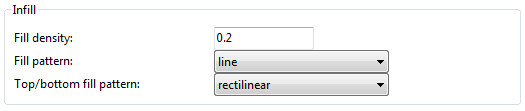
\includegraphics[keepaspectratio=true,width=1.0\textwidth]{expertmode/infill_pattern_settings.png}
\caption{R\'eglages des motifs de remplissage.}
\label{fig:infill_pattern_settings}
\end{figure}


Slic3r propose plusieurs mod\`eles de remplissage, quatre commun et trois variantes plus exotiques. Les chiffres indiqu\'es entre parenth\`eses sous chaque figure sont une estimation approximative du mat\'eriau utilis\'e et du temps pris pour un simple mod\`ele de 20 mm cube\footnote{Taken from http://gcode.ws}.  Notez que ce n'est qu'\`a titre indicatif, que la complexit\'e du mod\`ele et d'autres facteurs auront une incidence sur le temps et la mati\`ere.

\begin{figure}[H]
\centering
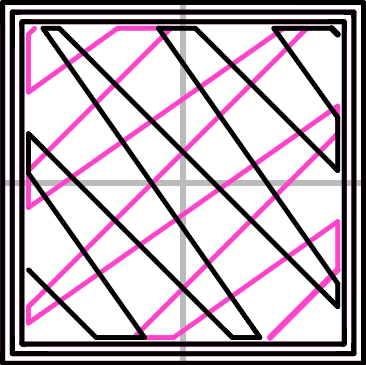
\includegraphics[keepaspectratio=true,width=0.2\textwidth]{expertmode/infill_line.png}
\caption{Motif de remplissage: Ligne (Line, 344.51mm / 5m:20s)}
\label{fig:infill_line}
\end{figure}

\begin{figure}[H]
\centering
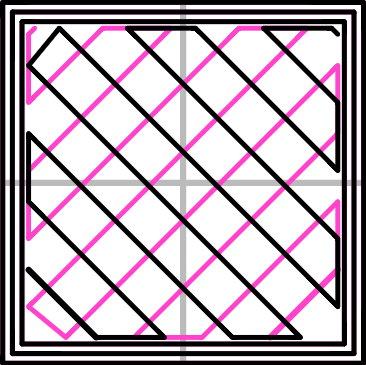
\includegraphics[keepaspectratio=true,width=0.2\textwidth]{expertmode/infill_rectilinear.png}
\caption{Motif de remplissage: Rectiligne (Rectilinear, 350.57mm / 5m:23s)}
\label{fig:infill_rectilinear}
\end{figure}

\begin{figure}[H]
\centering
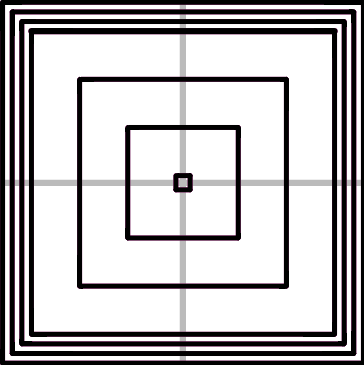
\includegraphics[keepaspectratio=true,width=0.2\textwidth]{expertmode/infill_concentric.png}
\caption{Motif de remplissage: Concentrique (Concentric, 351.80mm / 5m:30s)}
\label{fig:infill_concentric}
\end{figure}

\begin{figure}[H]
\centering
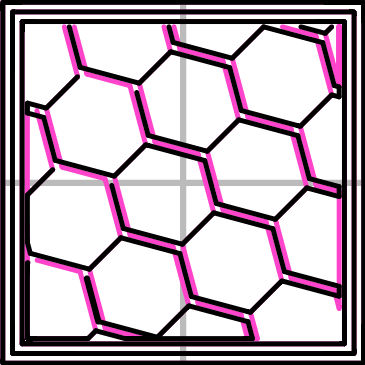
\includegraphics[keepaspectratio=true,width=0.2\textwidth]{expertmode/infill_honeycomb.png}
\caption{Motif de remplissage: Nid d'abeille (Honeycomb, 362.73mm / 5m:39s)}
\label{fig:infill_honeycomb}
\end{figure}

\begin{figure}[H]
\centering
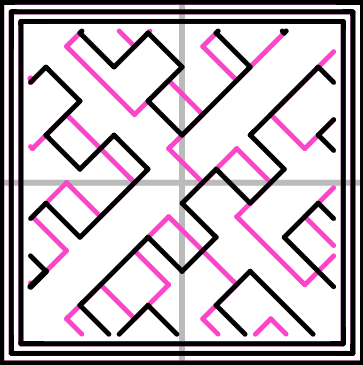
\includegraphics[keepaspectratio=true,width=0.2\textwidth]{expertmode/infill_hilbertcurve.png}
\caption{Motif de remplissage: Courbe de Hilbert (Hilbert Curve, 332.82mm / 5m:28s)}
\label{fig:infill_hilbertcurve}
\end{figure}

\begin{figure}[H]
\centering
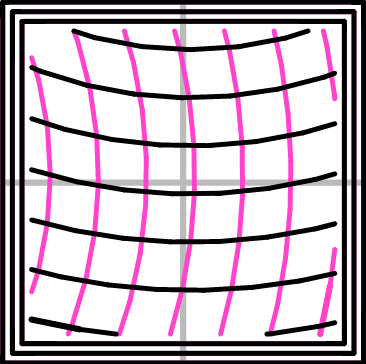
\includegraphics[keepaspectratio=true,width=0.2\textwidth]{expertmode/infill_archimedeanchords.png}
\caption{Motif de remplissage: Cordes d'Archim\`ede (Archimedean Chords, 333.66mm / 5m:27s)}
\label{fig:infill_archimedeanchords}
\end{figure}

\begin{figure}[H]
\centering
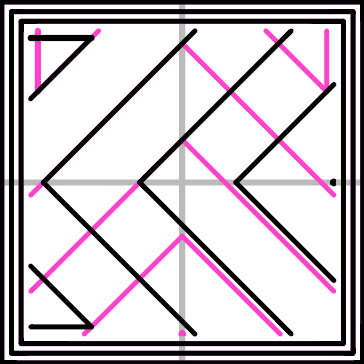
\includegraphics[keepaspectratio=true,width=0.2\textwidth]{expertmode/infill_octagramspiral.png}
\caption{Motif de remplissage: Spirale Octogramme (Octagram Spiral, 318.63mm / 5m:15s)}
\label{fig:infill_octagramspiral}
\end{figure}


Certains types de mod\`eles sont plus adapt\'es pour un motif particulier, par exemple le type organique par rapport au type m\'ecanique.  La figure \ref{fig:complex_object_infill_comparison} montre comment un remplissage en nid d'abeilles peut mieux convenir \`a cette pi\`ece m\'ecanique parce que chaque liaisons hexagonales avec la couche pr\'ec\'edente, forment une structure verticale solide.

\begin{figure}[H]
\centering
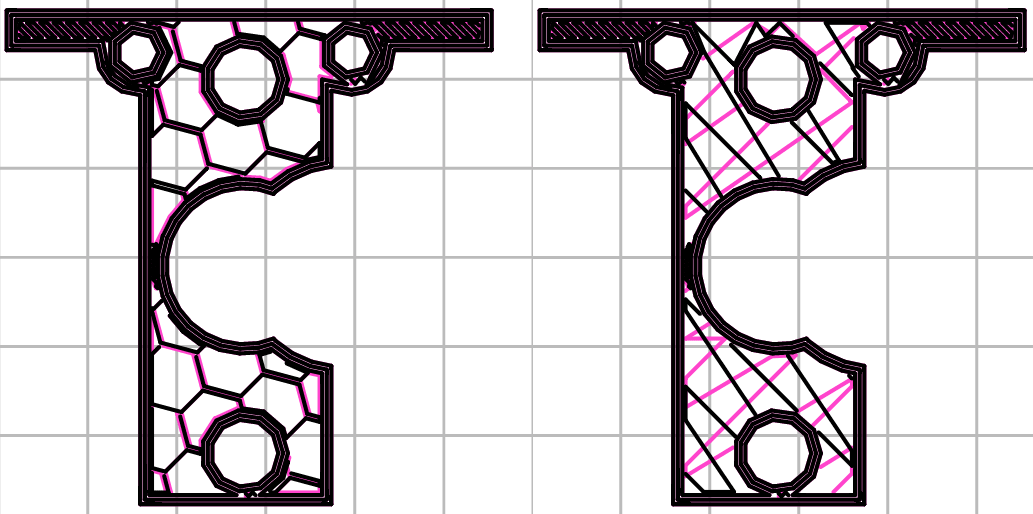
\includegraphics[keepaspectratio=true,width=0.75\textwidth]{expertmode/complex_object_infill_comparison.png}
\caption{Comparaison de motifs de remplissage pour un objet complexe. De gauche \`a droite: nid d'abeille, ligne}
\label{fig:complex_object_infill_comparison}
\end{figure}


La plupart des mod\`eles ne n\'ecessitent qu'un remplissage de faible densit\'e, en fournissant plus de, disons, 50\% produira un mod\`ele tr\`es serr\'es qui utilise plus de mati\`ere que n\'ecessaire. Pour cette raison, une gamme usuelle de r\'eglages est comprise entre 10\% et 30\%, mais les exigences du mod\`ele permettront de d\'eterminer o\`u la densit\'e sera la meilleure.  La figure \ref{fig:infill_pattern_densities} montre comment les motifs changent au fur et a mesure que la densit\'e augmente.
\begin{figure}[H]
\centering
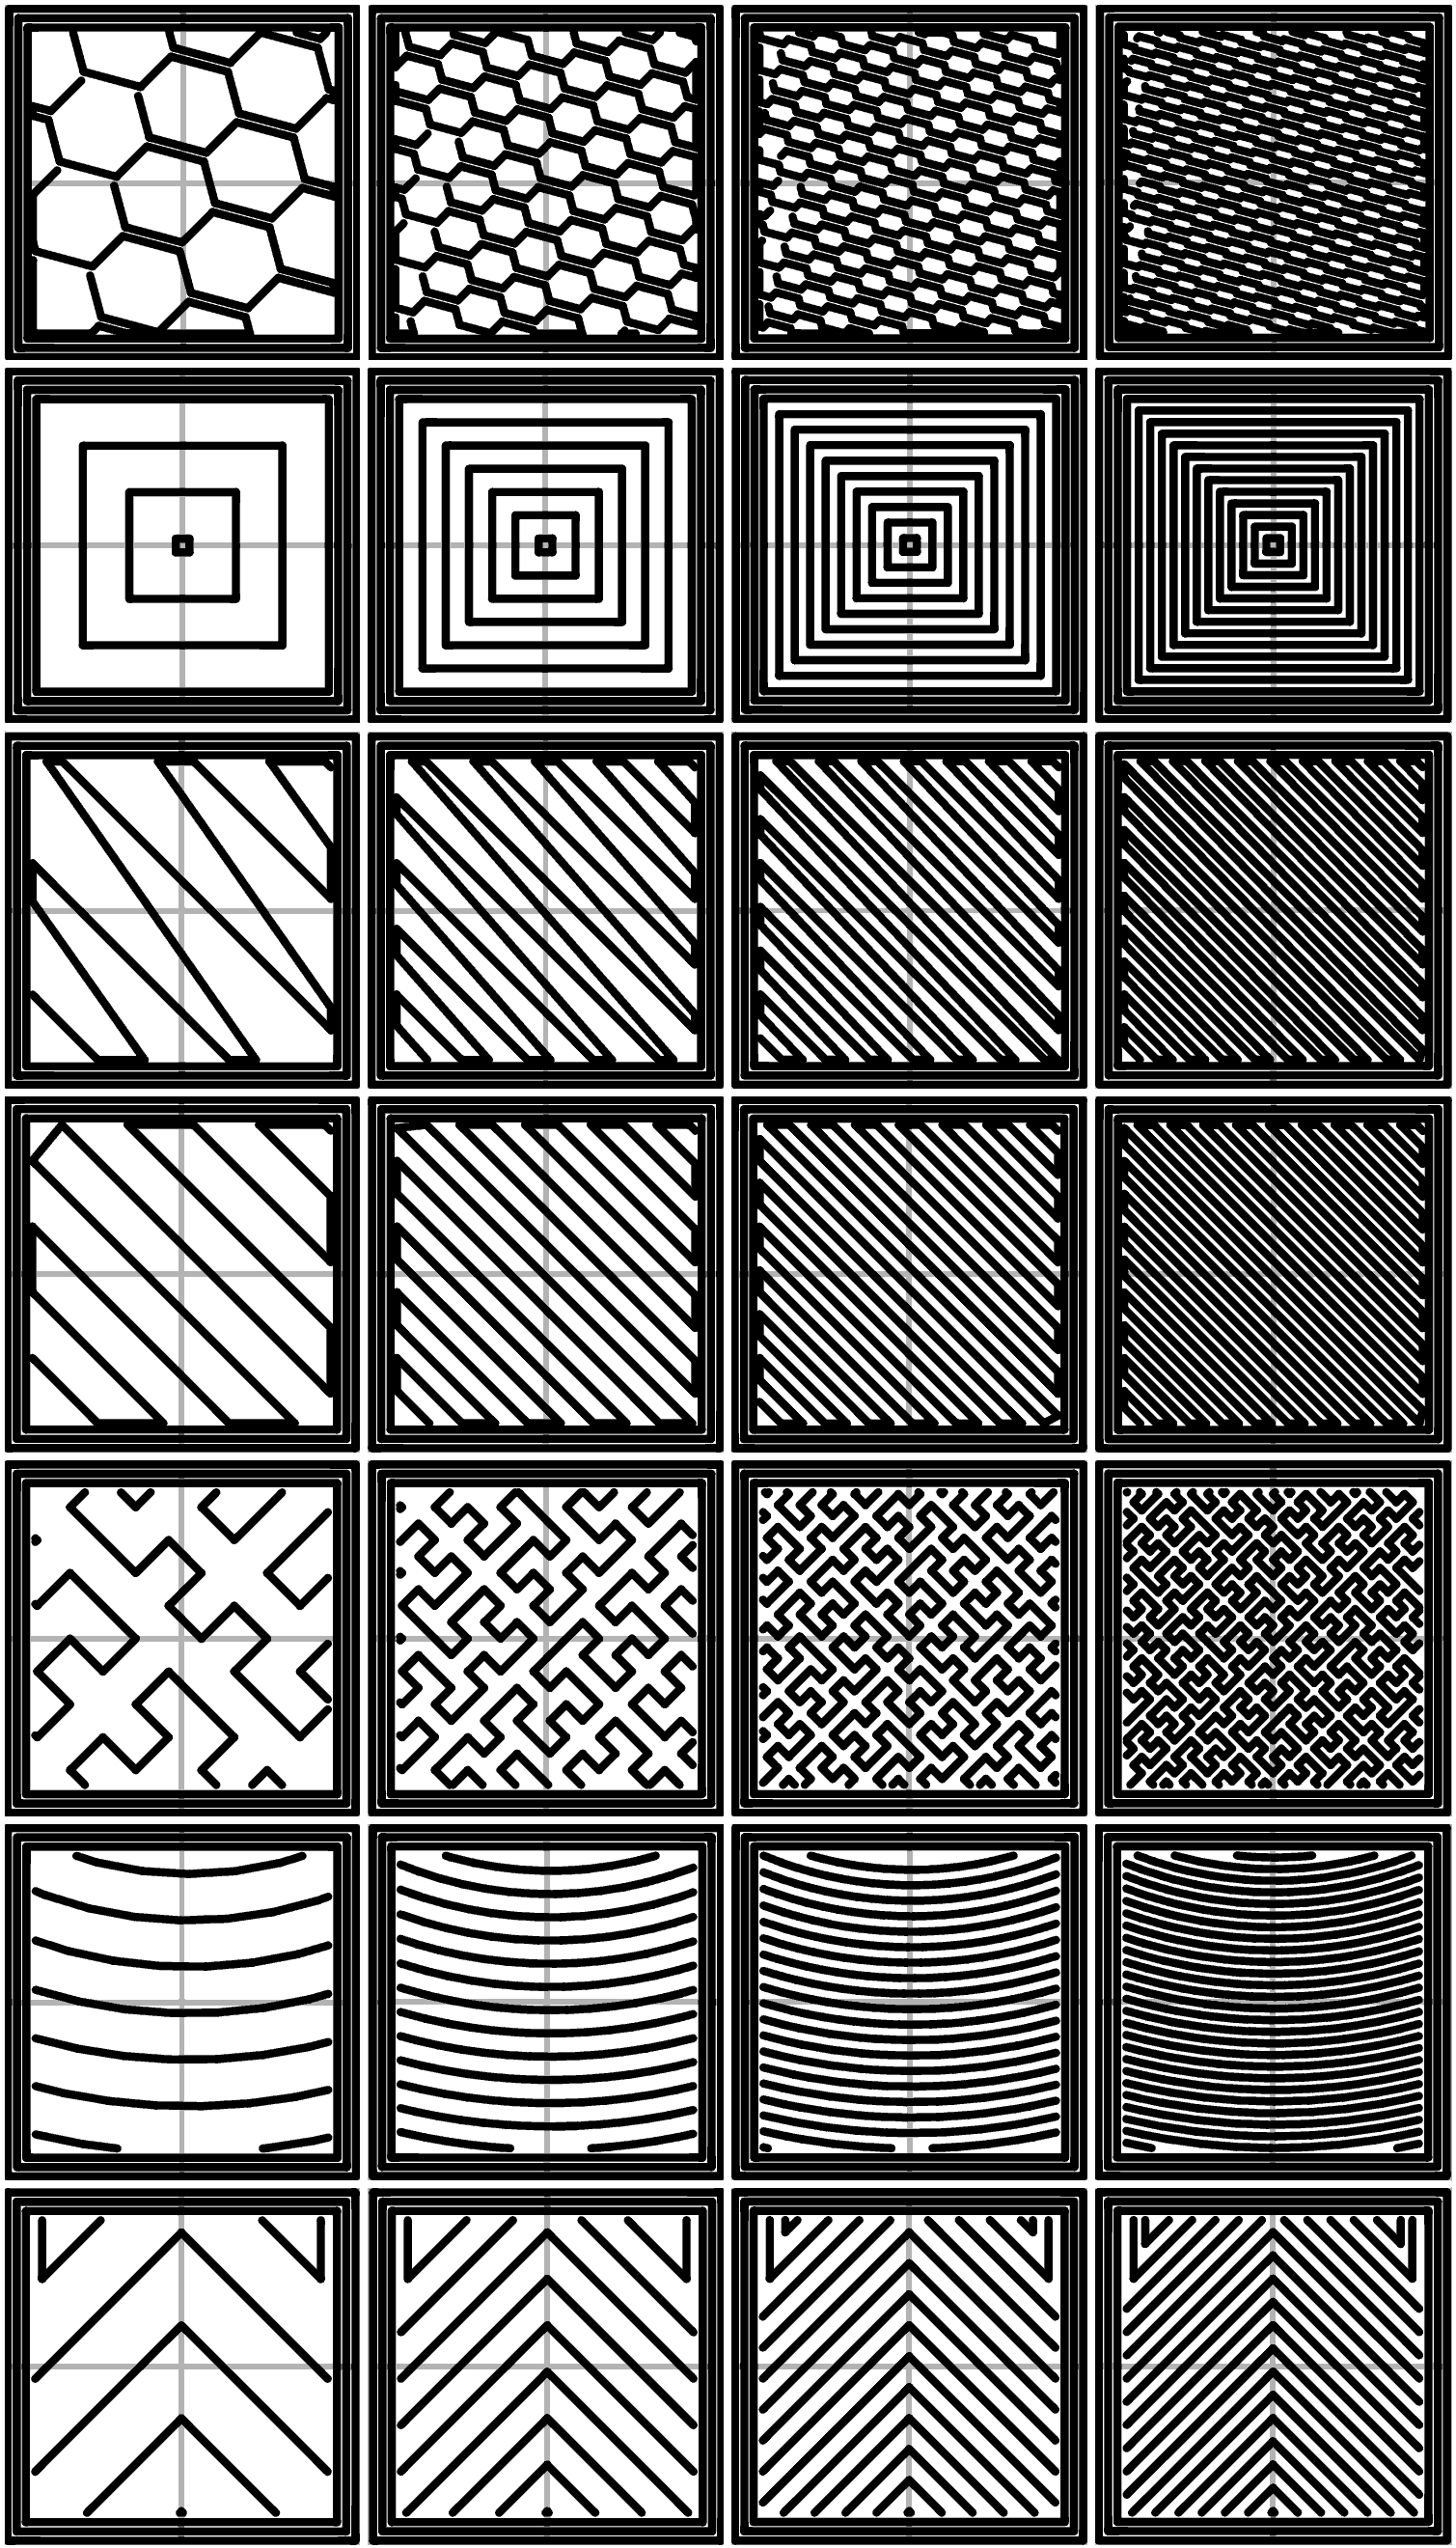
\includegraphics[keepaspectratio=true,width=0.7\textwidth]{expertmode/infills.png}
\caption{ Les motifs de remplissages \`a diff\'erentes densit\'es. de gauche \`a droite: 20\%,40\%,60\%,80\%. De haut en bas: Honeycomb, Concentric, Line, Rectilinear, Hilbert Curve, Archimedean Chords, Octagram Spiral}
\label{fig:infill_pattern_densities}
\end{figure}

% section infill_patterns_and_density (end)